\documentclass{article}

\usepackage{cs-296-proposal}
\usepackage{float}
\usepackage{amsmath} %for \text{}
\usepackage{amssymb}
\usepackage{graphicx}
\usepackage[toc,page]{appendix}
\usepackage{geometry}
\usepackage{eufrak}
\usepackage{fixltx2e}
\usepackage{bm}
\usepackage{tikz}
\usepackage{float}
\usepackage{xcolor}

\title{Reformulation, Extension, and Application \\ of the Formal Framework for P Systems}
\author{Ren Tristan A. de la Cruz}
\date{\today}

\documenttype{Thesis Proposal}
\degree{Doctor of Philosophy in Computer Science}
\proposaldate{2020 December 10}

\lab{Algorithms and Complexity Laboratory}
\dept{Department of Computer Science}
\college{College of Engineering}
\university{University of the Philippines}

\adviser{Francis George C. Cabarle, Ph.D.}
\coadviser{}
\memberone{}
\membertwo{}
\memberthree{}
\memberfour{}

\newcommand{\mn}{\text{-}}
\newcommand{\s}{\text{ }}
\newcommand{\ra}{\rightarrow}

%==================================================================================================%

\begin{document}

%==================================================================================================%

\maketitle

%==================================================================================================%

\begin{abstract}
\emph{Membrane computing} is a field of computer science that studies biologically-inspired 
parallel and distributed models of computations known as \emph{P systems}. At the moment, there
are hundreds of P systems variants with their own syntax and often informally defined semantics.
\emph{Formal framework} attempts to formally define a general syntax and procedural semantics for 
wide variety of P systems. This research proposal is about the reformulation, extension, and 
application of the said formal framework.
\end{abstract}

%==================================================================================================%

\newpage
\tableofcontents
\afterpreface

%==================================================================================================%

\section{Introduction}\label{s-intro}

\textit{Membrane computing} is a field of theoretical computer science that studies different models
of computation known as \textit{P systems}. The term `\textit{P systems}' refers to a family of 
models of computation which are inspired by biological processes. P system models use abstractions 
of biological processes as computational operations. For example, different types of rules 
(operations) used by most P system variants are abstractions of processes like \textit{chemical 
reaction} and \textit{ion transport} that occur inside biological cells. Most P system variants use 
\textit{object symbols} as the objects of computation. One can think of these object symbols as 
abstraction of physical \textit{molecules} or \textit{ions}. P systems store \textit{multisets} of 
these object symbols inside regions enclosed by \textit{membranes}. A P system has a collection of 
these membranes with multisets of objects symbols inside. The membranes can be `connected' to each 
other to form a \textit{membrane structure}. 

Aside from studying P systems themselves, membrane computing also deals with applications of 
P systems. P systems have been used to solve `hard' (NP-complete) problems. They have been used to 
model natural phenomena like biological oscillations, population dynamics, and sodium-potassium pump
mechanism. Other P system applications include boolean circuit simulation, fault diagnosis models
for electric locomotive, linguistic applications, etc.

There are tens, if not hundreds, of P system variants. Their syntax are well-defined but the 
semantics are often described in an informal manner. \emph{Formal framework} is an attempt to 
formalize not only syntax but also the procedural semantics of a wide variety of P systems. There
are currently three versions of the framework, one for P systems with static membrane structures,
one for P systems with dynamic membrane structures, and another for static P systems with 
input-output. The formal frameworks can be used to analyze, compared, and extended P systems.

The rest of the document can be divided into three parts. The first part, Section \ref{s-prelim}, 
describes P systems and formal frameworks in a semi-formal manner. The second part, Section
\ref{s-prop}, gives the proposal itself with the research objectives and schedule. The third part,
the Appendix, provides the full formal description of the formal frameworks. 

%==================================================================================================%

\section{Preliminaries} \label{s-prelim}

%==================================================================================================%

\subsection{P Systems}\label{s-psystem}

The following sections describe the components that are common to most (if not all) P system 
variants.

% ================================================================================================ %

\subsubsection{Membrane Structure}\label{s-membrane}

A P system has set of membranes that can be connected to each other. These connected membranes form
a \textit{membrane structure}. Early P systems are described as \textit{cell-like} since their 
membrane structures are inspired by nested membranes inside a cell. Figure \ref{fig:cell-like} shows 
an example of a cell-like membrane structure.

\begin{figure}[H]
\begin{center}
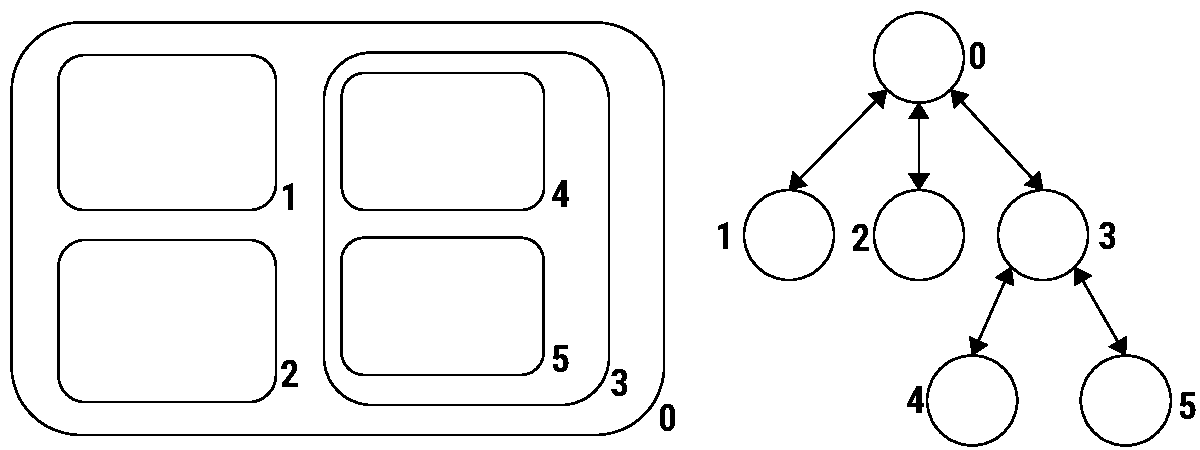
\includegraphics[scale=0.60]{figures/zzz-cell-like-structure.pdf}
\caption{Cell-like Membrane Structure}
\label{fig:cell-like}
\end{center}
\end{figure}

In Figure \ref{fig:cell-like} you can see two representations of a 6-membrane cell-like membrane 
structure. The left diagram shows the nesting of the membranes while right diagram shows the tree 
topology of the membranes. The outer most membrane, membrane 0, is the root node of the tree while 
membranes that do not contain internal membranes (membranes 1,2,4,5) are the leaf nodes of the tree.

Other P system variants use the more general graph membrane structure. P systems described as
\textit{tissue-like} or \textit{neural-like} use graph membrane structures. In \textit{tissue-like}
P systems, the membranes are called \textit{cells} and the connected cells form a `\textit{tissue}'. 
In \textit{neural-like} P systems, the membranes are called \textit{neurons} and the connected 
neurons form a \textit{neural network}. Figure \ref{fig:graph-topology} shows an example of a graph
membrane structure with 7 membranes.

\begin{figure}[H]
\begin{center}
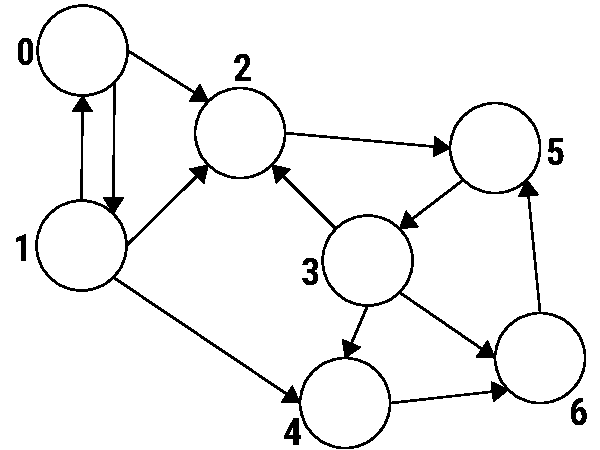
\includegraphics[scale=0.60]{figures/zzz-graph-topology.pdf}
\caption{Graph Membrane Structure}
\label{fig:graph-topology}
\end{center}
\end{figure}

% ================================================================================================ %

\subsubsection{Multisets of Object Symbols}\label{s-multiset}

As mentioned in Section \ref{s-intro}, the objects of computation in P systems are abstract
object symbols. Any P system has a fixed set of object symbols or an \textit{alphabet}. We denote 
this alphabet of object symbols as $V$. A multiset over alphabet $V$ is simply a set of object 
symbols from $V$ in which multiple instances of the same object symbols are allowed. For example, 
given the alphabet $V = \{a,b,c,d\}$, the following are some multisets over $V$:

\begin{itemize}
\item $\{a,a,b\}$
\item $\{a,a,b,c,c,d\}$
\item $\{c,d,d\}$
\item $\{a,c,c,c,d,d\}$
\item $\{a,a,b,b,b,c,c,c,c,d,d,d,d,d\}$
\end{itemize}

Multisets can be written as strings. For example:

\begin{itemize}
\item $\{a,a,b\} = aab = a^2b$
\item $\{a,a,b,c,c,d\} = aabccd = a^2bc^2d$
\item $\{c,d,d\} = cdd = cd^2$
\item $\{a,c,c,c,d,d\} = acccdd = ac^3d^2$
\item $\{a,a,b,b,b,c,c,c,c,d,d,d,d,d\}= aabbbccccddddd=a^2b^3c^4d^5$
\end{itemize}

In a P system, regions enclosed by membranes store multisets of object symbols. Figure 
\ref{fig:multisets-on-membranes} shows two examples of membrane structures (cell-like and graph) 
with multisets of symbols in the  regions.

\begin{figure}[H]
\begin{center}
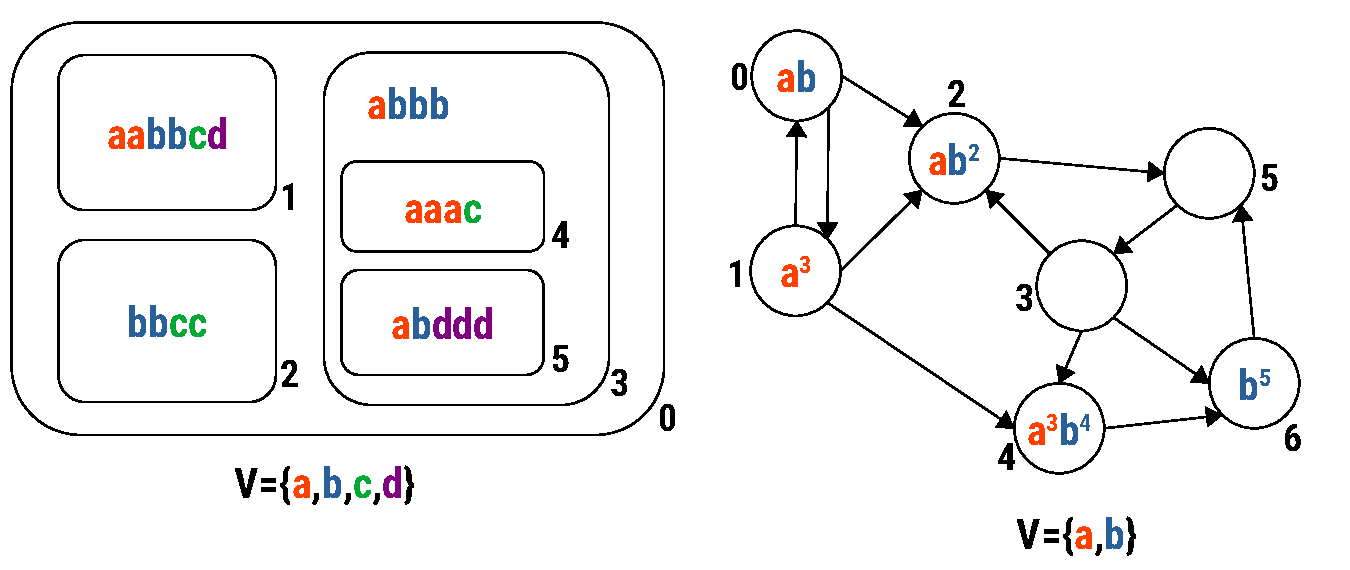
\includegraphics[scale=0.55]{figures/zzz-multisets-on-membranes.pdf}
\caption{Multisets in Membrane Structures}
\label{fig:multisets-on-membranes}
\end{center}
\end{figure}

The left diagram in Figure \ref{fig:multisets-on-membranes} shows the membrane structure from Figure
\ref{fig:cell-like} with multisets over alphabet $V=\{a,b,c,d\}$. Membrane 0 is empty (or contains 
the empty multiset). Membrane 1 contains the multiset $aabbcd$. Membrane 2 contains the multiset
$bbcc$. Membrane 3 contains the multiset $abbb$, etc. The right digram in Figure 
\ref{fig:multisets-on-membranes} shows the membrane structure from Figure \ref{fig:graph-topology} 
with multisets over alphabet $V=\{a,b\}$. Cell 0 contains the multiset $ab$. Cell 1 contains the 
multiset $a^3$. Cell 2 contains the multiset $ab^2$. Cell 3 is empty, etc. 

% ================================================================================================ %

\subsubsection{Rules of Different Types}\label{s-rule}

A P system uses a set of rules to perform computation. Different P system variants use different
types of rules. In general, a rule transforms the multisets inside the membranes and/or transforms
the membrane structure itself. Static structure P systems only use rules that primarily
transform the multisets inside the membranes and do not change the structure of the system. Dynamic
structure P systems have rules that can add new membranes, delete existing membranes, and change the
connections between membranes.

Rules for transforming multisets inside the membranes are based on \textit{multiset rewriting 
rules}. A \textit{multiset rewriting rule} is written as $M \rightarrow M'$ where $M$ and $M'$ are 
both multisets over the same alphabet. The rule rewrites the multiset $M$ to the multiset $M'$.

For example: Alphabet is $V = \{a,b,c,d\}$

\begin{itemize}

\item \texttt{Rule 1}: $a^2b^2 \rightarrow cd$
\begin{itemize}
\item Applying \texttt{Rule 1} once to multiset $a^4b^5c^3d^2$ will transform it to $a^2b^3c^4d^3$.
\item Applying \texttt{Rule 1} twice to multiset $a^4b^5c^3d^2$ will transform it to $bc^5d^4$.
\end{itemize}

\item \texttt{Rule 2}: $ad \rightarrow ab^2c^3$
\begin{itemize}
\item Applying \texttt{Rule 2} once to multiset $a^4b^5c^3d^2$ will transform it to $a^4b^7c^6d$.
\item Applying \texttt{Rule 2} twice to multiset $a^4b^5c^3d^2$ will transform it to $a^4b^9c^9$.
\end{itemize}

\end{itemize}

The first P system, known as \textit{transition P system} \cite{comp-w-mem}, is a cell-like P system
that uses modified multiset rewriting rules. Rules in transition P systems are multiset rewriting 
rules that use the membrane structures of the systems. A rule is associated with the region enclosed
by a specific membrane. A rule will `consume' a multiset of object symbols in its region then it can
produce multisets of object symbols in the same (\textit{here}) region, in the region outside 
(\textit{out}) its membrane, and/or in the regions enclosed by membranes inside (\textit{in}) the
rule's own membrane. Figure \ref{fig:trans-rule} shows an example of a rule being applied.

\begin{figure}[H]
\begin{center}
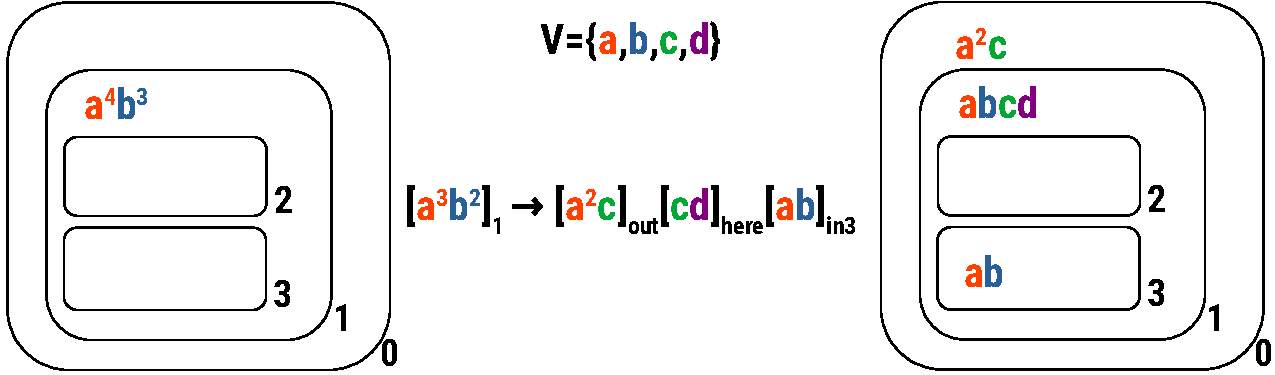
\includegraphics[scale=0.55]{figures/zzz-transition-rule.pdf}
\caption{Application of Transition Rule $[a^3b^2]_1 \rightarrow [a^2c]_{out}[cd]_{here}[ab]_{in_3}$}
\label{fig:trans-rule}
\end{center}
\end{figure}

The left diagram on Figure \ref{fig:trans-rule} shows the \textit{configuration} of the system
before rule application. Membrane 1 contains the multiset $a^4b^3$ while the other membranes are 
empty. The rule $[a^3b^2]_1 \rightarrow [a^2c]_{out}[cd]_{here}[ab]_{in_3}$ is associated with the
region  enclosed by membrane 1. The rule consumes $a^3b^2$ from membrane 1, produces $a^2c$ outside 
membrane 1 (in membrane 0), and produces $ab$ inside membrane 3. The right diagram on Figure 
\ref{fig:trans-rule} shows the configuration of the system after the rule is applied.

It can also be specified in a rule in a transition P system that the membrane associated with the 
rule be \textit{dissolved} after the rule was applied. Figure \ref{fig:trans-rule2} shows how a rule
can \textit{dissolve} a membrane. Rule $[a^2b^2]_1 \rightarrow [ab]_{in_2}[cd]_{in_3}\delta$ 
consumes multiset $a^2b^2$ from membrane 1, produces multiset $ab$ in membrane $2$, produces 
multiset $cd$ in membrane 3, and \textit{dissolves} membrane 1 (this is specified by $\delta$ at the
end of the rule). The remaining multiset in membrane 1 will go to its parent membrane, membrane 0.

\begin{figure}[H]
\begin{center}
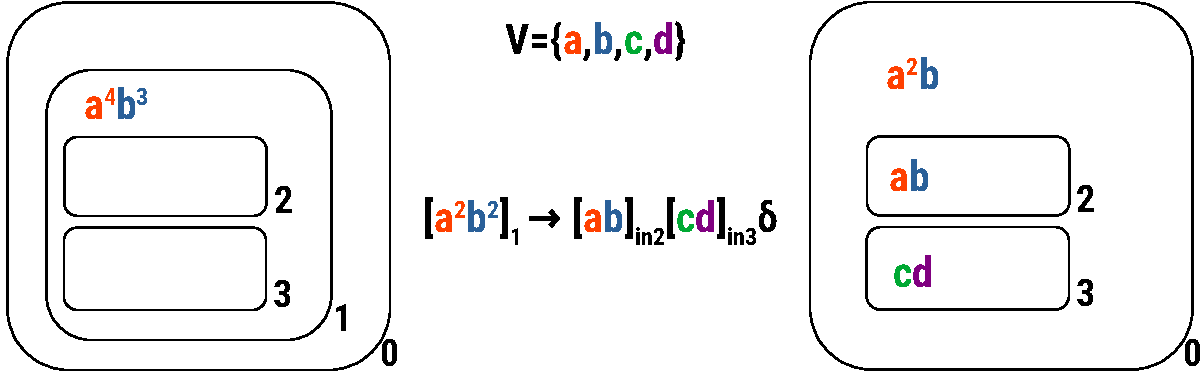
\includegraphics[scale=0.55]{figures/zzz-transition-rule2.pdf}
\caption{Application of Transition Rule $[a^2b^2]_1 \rightarrow [ab]_{in_2}[cd]_{in_3}\delta$}
\label{fig:trans-rule2}
\end{center}
\end{figure}

\textit{Tissue P systems}' \cite{tissue-p} rules are very similar to rules in transition P systems. 
The difference is that tissue P systems' membrane structures form graphs that do not have
directionality or orientation unlike the tree membrane structures of transition P systems. When you
are in the node of a tree in the membrane structure of a transition P system, the rule can send 
produced multisets \textit{out} in the direction of the parent node, in the same node 
(\textit{here}), or in the direction of the children nodes (\textit{in}). In tissue P systems, a 
rule can send produced multisets in the same node (\textit{here}) or to the adjacent nodes 
(\textit{out}). Aside from this rule convention, rules in tissue P systems also have multiple 
different semantic meanings.

\begin{figure}[H]
\begin{center}
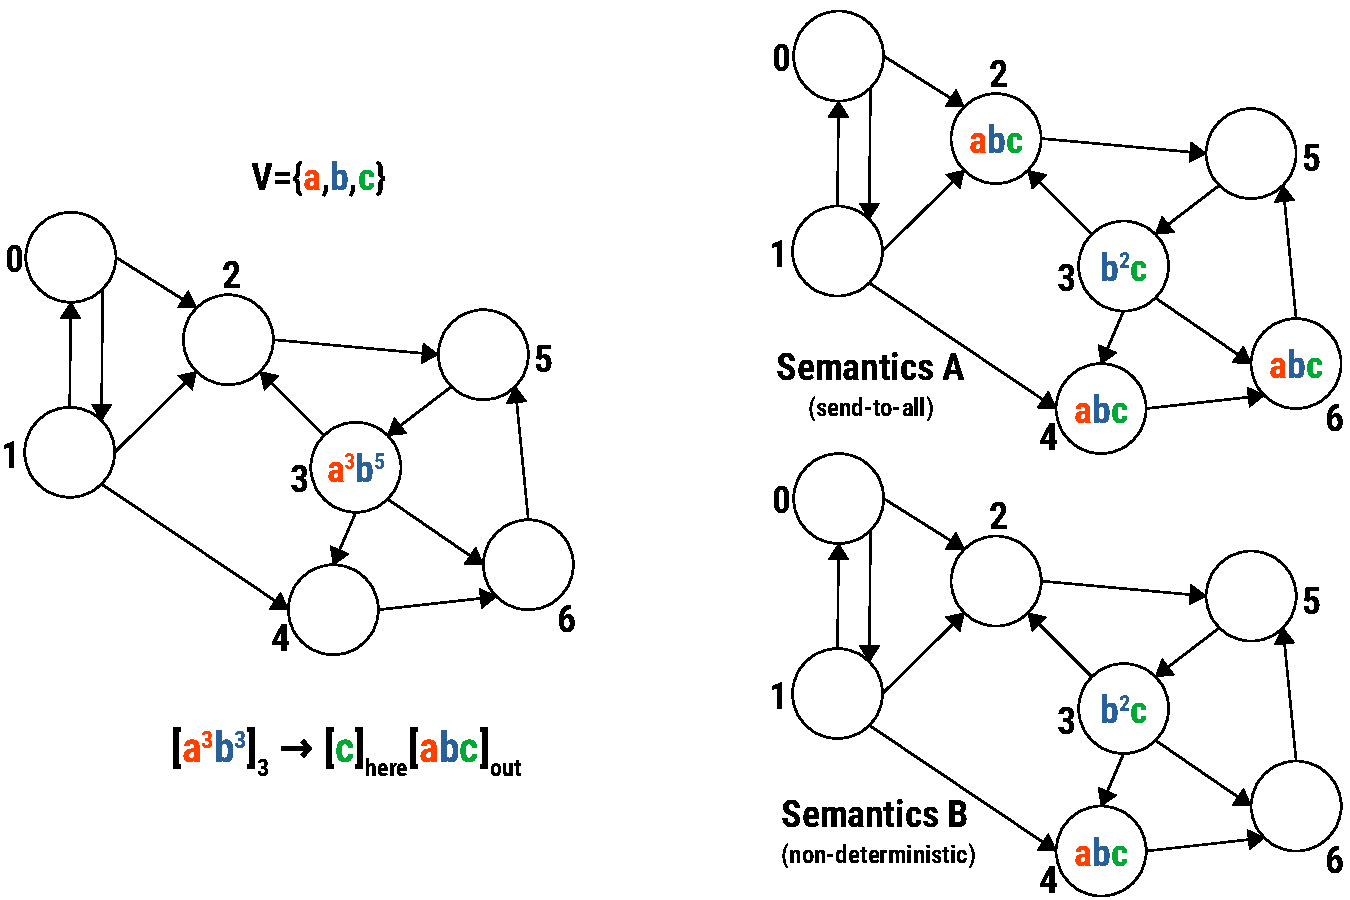
\includegraphics[scale=0.55]{figures/zzz-tissue-rule.pdf}
\caption{Application of Tissue P system Rule $[a^3b^3]_3 \rightarrow [c]_{here}[abc]_{out}$}
\label{fig:tissue-rule}
\end{center}
\end{figure}

Figure \ref{fig:tissue-rule} shows two interpretations (Semantics A and B) for the rule 
$[a^3b^3]_3 \rightarrow [c]_{here}[abc]_{out}$. For semantics A, the rule consumes multiset 
$a^3b^3$ from cell 3, produces multiset $c$ in cell 3, and sends multiset $abc$ to all adjacent
cells (cells 2,4,6). For semantics B, the rule consumes multiset $a^3b^3$ from cell 3, produces
multiset $c$ in cell 3, and \textit{nondeterministically} sends multiset $abc$ to one of the
cells adjacent to cell 3 (either cell 2,4, or 6).

P systems \textit{with active membranes} \cite{active-mem} introduced a type of rule that allows
creation of new membranes. Figure \ref{fig:active-mem-rule} shows a rule of this type. The rule 
$[a]_y \rightarrow [b]_y[c]_y$ in Figure \ref{fig:active-mem-rule} has a very similar syntax to 
previous rules but its semantics is different. The rule consumes the object symbol $a$ in membrane 
labeled $y$. The rule will then duplicate the membrane copying all the remaining object symbols to
both membrane copies. Both membrane copies are also labeled $y$. In this P system variant, membrane 
labels are not membrane ids so multiple membranes can have the same label. In one of the copies, 
object symbol $b$ is produce while in the other copy object symbol $c$ is produced. Figure
\ref{fig:active-mem-rule} shows the rule being applied twice in two steps.

\begin{figure}[H]
\begin{center}
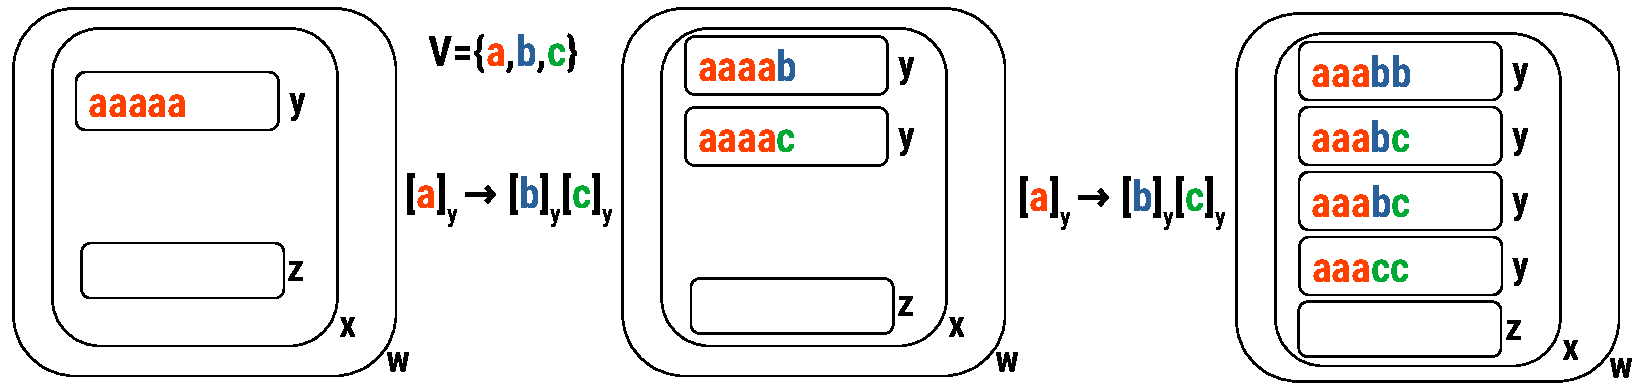
\includegraphics[scale=0.55]{figures/zzz-active-mem-rule.pdf}
\caption{Application of the Active Membrane Rule $[a]_y \rightarrow [b]_y[c]_y$}
\label{fig:active-mem-rule}
\end{center}
\end{figure}

The types of rules described above form a small set of samples of all possible types of rules. A 
large portion of the other types of rules that are not discussed are variations of the rules 
above. Some of them may have a slightly different semantics to the rules above.

% ================================================================================================ %

\subsubsection{Derivation Modes}\label{s-semantics}

P systems are parallel computing models. A P system can apply multiple rules at the same time.
Different P systems can have different conventions that say which combinations of rules can be 
applied at the same time. This convention is known as the \textit{derivation mode} of the system.
A common derivation mode is called \textit{maximally parallel} derivation mode. In maximally
parallel mode, the system will apply a combination of rules such that you can no longer add 
instances of rules to this \textit{maximal} combination of rules. For example, you have:

\begin{itemize}
\item \texttt{Rule 1:} $[ab]_1 \rightarrow [xy]_{here}$
\item \texttt{Rule 2:} $[b^2]_1 \rightarrow [xyz]_{here}$ 
\end{itemize}

\texttt{Rule 1} consumes $ab$ from membrane 1 while \texttt{Rule 2} consumes $b^2$
from membrane 1. If membrane 1 contains the multiset $a^3b^6$, one maximal combination of rules is
$3 \times$\texttt{Rule 1} + \texttt{Rule 2}. This combination will consume the multiset $a^3b^5$.
With the multiset $b$ remaining no additional rules can be added to the combination making the
combination maximal. Another maximal combination of rules is $3\times$\texttt{Rule 2}. This
combination will consume the multiset $b^6$. With the multiset $a^3$ remaining no additional rules
can be added. Another maximal combination is $2\times$\texttt{(Rule 1 + Rule 2)} consuming the
multiset $a^2b^6$. In maximally parallel mode, only a maximal combination of rules can be applied.
For example, the system can not apply the combination with one instance of \texttt{Rule 1}, if the
system can still apply additional rules then it will add these rules to the combination. In this
mode, the system \textit{maximizes} the rules it can apply.

\textit{Minimally parallel} mode is often used in \textit{neural-like} P system variants. In the
minimally parallel mode, at most one applicable rule is applied per membrane. The `parallel' part is
that multiple membranes can apply a rule at the same time. The `minimal' part is that at most one
rule can be applied per membrane.

There are other derivations modes. Some P system variants have the same rule types and membrane
structure but only differ in the derivation modes they use.

%==================================================================================================%

\subsection{Formal Framework}

The \emph{first formal framework (FF1)} \cite{ff-static} is an attempt to formally define procedural
semantics for a large number of well-known variants of tissue P systems with static membrane 
structures. The \emph{second formal framework (FF2)} \cite{ff-dynamic} is a similar attempt for P 
systems with dynamic membrane structures. The \emph{third formal framework (FF3)} \cite{ff-snp} is 
an extension of FF1 with the purpose of expressing spiking neural P systems \cite{snp} in this
extended framework.

The formal frameworks use and formalize notions/concepts common to most of their target P systems.
The main notions available in all three versions of the framework are the following: 

\begin{enumerate}
\item \emph{configuration} of the system
\item \emph{rules} of the system
\item \emph{applicability} of a combination of rules
\item \emph{allowed} combinations of rules
\item how to \emph{apply} a combination of rules
\item \emph{halting} condition for the system 
\end{enumerate}

%==================================================================================================%

\subsubsection{Configuration}

In FF1, the \emph{configuration} of the system can be represented by a fixed-size vector of 
multisets $C = (u'_1,...,u'_n)$, $u'_i$ being the multiset in cell $i$. The configuration in FF1
does not contain information about the connections between cells. Instead, the information about the 
connection between cells is embedded in the rules themselves. For example, \texttt{Rule 1} is a rule
that transfers objects from cell $A$ to cell $B$  therefore it requires a connection between cell 
$A$ and cell $B$. Since FF1 deals only with static membrane structure, if there is no connection
between cell $A$ and cell $B$ then \texttt{Rule 1} is useless in the system. In FF1, if a rule is in
the system and it requires certain connections between cells, then it is implied that those
connections exist in the system. For a static system, you only need the vector of multisets (of the
cells) in order to define the configuration of the system since the multisets are the only ones that
can change. FF3 has the same configuration.

In FF2, the configuration $\mathcal{C}$ of the system is defined by the pair $ (L, \rho)$. $L = 
\{(i_1,l_1,w_1),...,(i_n,l_n,w_n)\}$ is a list of labeled cells. The triple $(i_j,l_j,w_j)$ is a 
cell with id $i_j$, label $l_j$, and multiset $w_j$. $\rho$ is a set of cell id pairs that represent
the connections between cells. $L$ can change not only by changing the labels or contents of the 
cells in the list but also by adding/removing cells to/from the list. $\rho$ can also change by 
adding or removing connections (pair of cell ids) between cells.

In some P system variants like P systems with active membranes \cite{active-mem}, cells have 
additional properties that can change throughout the computation. For example, the cells in P 
systems with active membranes have a \emph{charge/polarity} property that can either be $+$ 
(positive), $-$ (negative), or $0$ (neutral). Such properties can be represented by adding extra
symbols to the system's alphabet. Using this technique of adding extra symbols, FF1 and FF2's 
configurations can already represent most of these additional cell properties.

For the full technical details on how a configuration is defined in FF1 see Appendix 
\ref{a-ff1-config} and see Appendix \ref{a-ff2-config} for the details on how a configuration is 
defined in FF2. Configuration for FF3 is the same as configuration in FF1.

%==================================================================================================%

\subsubsection{Interaction Rules}

In all three FFs, the system's rules are referred to as \emph{interaction rules}. In FF1, an 
\emph{interaction rule} has the form $(X \ra Y; P,Q)$. $X = (x_1,...,x_n)$ is a vector of multisets
where $x_i$ represents the multiset that will be \emph{consumed} in cell $i$ if the rule is used.
$Y = (y_1,...,y_n)$ is a vector of multisets where $y_j$ is the multiset that will be 
\emph{produced} in cell $j$ if the rule is used. $P = (p_1,...,p_n)$ is a vector of sets of 
multisets where $p_i$ contains different multisets (\emph{permitting conditions}) that should be in 
cell $i$ for the rule to be \emph{eligible}. We will elaborate on the concept of \emph{rule 
eligibility} in the Section \ref{s-applicable}. $Q = (q_1,...,p_n)$ is a vector of sets of multisets
where $q_i$ contains different multisets  (\emph{forbidding condition}) that should not be in cell 
$i$ for the rule to be eligible. The notation $X\ra Y$ means the multisets in $X$ are 
\emph{rewritten} as the multisets in $Y$.

The interaction rules in FF3 (see Appendix \ref{a-ff3}.\ref{a-ff3-rule}) has a very similar form
to the interaction rule in FF1. The difference is that rules in FF3 use a vector of regular 
expressions $E = (E_1,...,E_i,...,E_n)$ as \emph{permitting conditions} and there are not forbidding
conditions. The semantics of the rules related to these regular expression is particular to spiking
neural P system variants.

For FF1 and FF2, a form of multiset rewriting rule is sufficient. For FF2, changes in the membrane 
structure should also be capture by the rule. An interaction rule in FF2 has the form: 
$$r=(Label, \rho, Perm, For, Rewrite, Label\mn Rename, Delete, $$ $$Delete\mn and\mn Move,Generate, 
Generate\mn and \mn Copy, Change\mn Relation)$$ 
Aside from multiset rewriting, a rule in P systems with dynamic membrane structures can also create
new membranes, delete existing membranes, and change connections between membranes. This is the
reason why a rule in FF2 has 11 components. The component $label$ specifies the labels of the
cells the rule is concerned with. The component $\rho$ specifies the connection needed for the rule
to be \emph{eligible}. The components $Perm$ (permitting conditions), $For$ (forbidding conditions),
and $Rewrite$ (rewriting rule) are similar to the components of the interaction rule for FF1. They 
specify conditions for rewriting the multisets and the rewriting rule itself. The component 
$Label\mn Rename$ specifies the some cells new labels. The component $Delete$ specifies the cells 
(and contained multisets) to be deleted. The component $Delete\mn and\mn Move$  specifies the cells
that will be deleted but whose contents will be moved to other cells. The component $Generate$ 
specifies the new cells (with new content) that will be created while the component $Generate\mn and
\mn Copy$ specifies new cells that will be created whose content will be rewritten version of copies
of multisets from existing cells. The component $Change\mn Relation$ specifies that changes to the 
connections between cells. Complete description for a FF2 interaction rule is in Appendix 
\ref{a-ff2-rule}.

%==================================================================================================%

\subsubsection{Applicability of a Multiset of Rules} \label{s-applicable}

P systems are parallel models of computation. Multiple rules associated with different membranes can
be applied in parallel. It is also possible for a single rule to be applied multiple times at the 
same time as shown in Section \ref{s-rule}. Taking the set of rules as the alphabet, the 
\emph{combination} of rules in Section \ref{s-rule} actually refers to a multiset over the set of
rules or simply a multiset of rules. 

Informally, the notion of the \emph{applicability} of a multiset of rules means that each rule in
the multiset can be applied a specified number of times (defined by the multiset) at the same time.
For example, applying the multiset ${r_1}^3{r_2}^5{r_5}^2$ means applying rule $r_1$ three times, 
rule $r_2$ five times, and rule $r_5$ two times. The multiset ${r_1}^3{r_2}^5{r_5}^2$ is applicable
if applying all the rules will not cause issues like needing to consume more objects than the cells
can provide. For example, if a rule $r_1$ consumes $ab$ from cell $1$ and cell $1$ contains the 
multiset $a^3b^{10}$, multiset ${r_1}^4$ is not applicable since the multiset needs to consume $a^4$
from cell 1 but cell 1 only has $a^3$ to provide.  The FFs formalized this notion of 
\emph{applicability}.

The FFs starts with the notion of \emph{eligibility} of a rule. In FF1, a rule 
$r:(X \ra Y;P,Q)$ is eligible if three conditions hold: (1) multisets $x_i$ in $X$ are contained by 
the multisets $u'_i$ in the cells, $x_i \subseteq u'_i$, (2) for each cell $i$, the set of 
permitting conditions $p_i$ in $P$ contains multisets that should be contained by multiset $u'_i$ of 
cell $i$,  $\forall p \in p_i,\s p \subseteq u'_i$, (3) for each cell $i$, the set of forbidding
conditions $q_i$ in $Q$ contains multisets that should not be contained by multiset $u'_i$ of cell
$i$, $\forall q \in q_i,\s q \not\subseteq u'_i$. The first condition checks if there are enough
objects in the cells for the rule to consume. The second condition checks for permitting conditions
for each cell. The third conditions checks for forbidding conditions for for each cell.

FF2 has the same 3 conditions for rule eligibility. These 3 conditions can be check using FF2 rule's
$Perm$, $For$, and $Rewrite$ components. Aside from these 3 conditions, for FF2 rule eligibility the
necessary $labels$ and connections $\rho$ should be available in the system's configuration 
$\mathcal{C}=(L, \rho)$.

The notion of rule eligibility can be extended to applicability of a multiset of rules by
simply adding the condition that there are enough objects in the cells for the rules to consume 
(consumption condition). In FF2, two additional conditions are (1) the label renaming components of 
the rules should not conflict with each other (i.e. a conflict would be rule $r_1$ relabelling cell 
$i$ with label $l$ while $r_2$ relabelling cell $i$ with label $l'$), (2) the $Change\mn Relation$ 
component of the rules should be commutative (i.e. rule $r_1$ applying its changes to the cell 
connections followed by rule $r_2$ applying its changes to the cell connections should result to the
same final set of connections if the order of rule applications is reversed). 

Full details for checking applicability of multiset of rules is in Appendix \ref{a-ff1-applicable}
for FF1/FF3 and in Appendix \ref{a-ff2-applicable} for FF2.

\subsubsection{Derivation Modes}

If multiset of rules $R$ is applicable, it is not necessarily the case that it is a candidate for
the multiset that will be applied to the system. There is an additional consideration known as the 
\emph{derivation mode}. The derivation mode of the system tells which of the applicable multisets 
of rules are candidate to be applied to the systems. Some of the common derivation modes are listed
below: 

\begin{itemize}
\item \emph{Sequential:} This derivation mode requires the system to apply at most one rule once at
       a time hence the word \emph{sequential}. This means the only candidate multisets for 
       application are the multisets with one rule that is applied once.
\item \emph{Asynchronous:} This derivation mode is the most flexible by allowing any applicable 
       multisets of rules to be a candidate.
\item \emph{Maximally parallel:} This derivation mode requires the candidate multiset to be 
      \emph{maximal} which means no additional rules can be added to the multiset without breaking 
      the object consumption condition for applicability of the multiset of rules.
\item \emph{Minimally parallel:} This derivation mode requires the candidate multiset to have some
       minimal level of parallelism. For example, the set of rules is partitioned and each partition
       of rules is associated with a membrane. A candidate multiset of rules is minimally parallel
       if for each partition of rules at most one rule in the partition appears in the candidate 
       multiset and is only applied once. In this example, at most one rule can be applied once per
       membrane. 
\end{itemize}

The formal definitions of the derivation modes above are available in Appendix \ref{a-ff1-derive}.
The appendix also contains additional derivation modes. These derivation modes are available to all
FFs.

%==================================================================================================%

\subsubsection{Halting Conditions}

Halting condition specifies criteria to tell if the system is in the halt state. Three halting 
conditions are defined in FF1 (see Appendix \ref{a-ff1-halt} for details).

\begin{itemize}
\item \emph{Total Halting} is the most common halting condition. It states that the system halts if
       there is no applicable multiset of rules. 
\item \emph{Adult Halting} says that the system is in the halt state if there are still applicable 
      multisets of rules but applying any of these to the system's current configuration will 
      simply result to the same configuration. The system is basically stuck applying those rules 
      without changing its configuration.
\item \emph{Partial Halting} is where you consider the system in halt state if there are still
      applicable multisets of rule but none of the applicable multisets contain one rule from each
      of the partitions of rules.
\end{itemize}

%==================================================================================================%

\subsubsection{Additional Notions in FF3}

Spiking neural P systems and many of its variants are often used as transducers that accept input
signals and produce output signals. The signals are known as \emph{spike trains}. For this reason, 
the formal framework for spiking neural P systems formalized the notions of SN P system's input and 
output. FF3 (see Appendix \ref{a-ff3}) defines the $Input$ function and the $Output$ function to 
formalized the input and output notions respectively.

The $Input$ function's purpose is to produce a size $n$ vector of multisets, $n$ being the number of
cells in the system. The $Input$ function takes a time parameter which specifies the current 
computation step. The function will then return the input vector of multisets for that given time. 
At time $t$, if cell $i$ is an input cell then the $i^{th}$ element of the input vector is the 
multiset input for cell $i$ at time $t$ otherwise if cell $i$ is not an input cell then the $i^{th}$ 
element of the input vector will be empty (the empty multiset).

The $Output$ function produces a size $n$ vector of multisets that represent the output of the
system. It takes time parameter $t$, the computation history $C(t) = C_0,...,C_t$ up to time $t$, 
and the ids of the output cells $c_{out}$ then it returns a size $n$ vector of multisets that is 
similar to configuration $C_t$ expect all the multisets which are not in the output cells 
($c_{out}$) will be set as empty multisets.

%==================================================================================================%

\subsubsection{Using the Formal Frameworks}

In \cite{ff-using}, both FF1 and FF2 were used to implement different features of P system variants.
These features include \emph{membrane thickness/polarity/labels}, \emph{rule priorities}, and
\emph{membrane dissolution}. P system variants like \emph{catalytic P systems}, \emph{P systems with 
symport/antiport} \cite{sym-anti-port}, \emph{P colonies}, and \emph{probabilistic P systems} were 
also implemented as specific FF models. \cite{ff-using} shows that the formal framework can be used 
to model a wide variety of P systems with diverse features and semantics.

The FF can be used to compare different P system variants. By translating P system variants to their
corresponding FF models, one can directly compare these FF models. The FF can be used a common 
language to analyze, compare and extended different P system variants.

%==================================================================================================%

\section{Proposal}\label{s-prop}

The research proposal has three aspects: (1) the reformulation of the formal framework, (2) the 
extension of the formal framework, and (3) the application of the formal framework. Figure 
\ref{fig:ff-p-system} shows the three aspects of the proposal.  

\begin{figure}[H]
\begin{center}
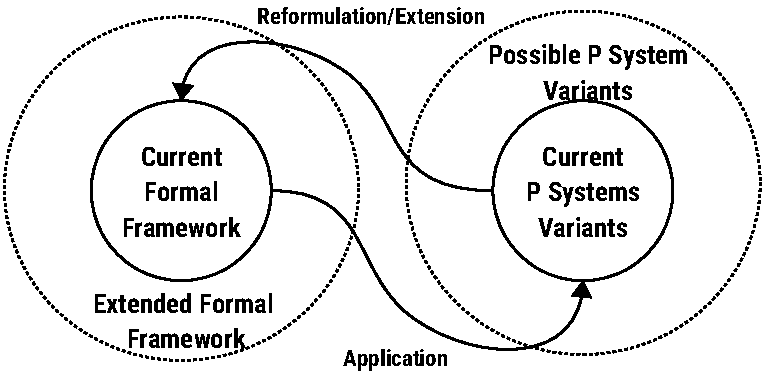
\includegraphics[scale=0.80]{figures/zzz-ff-p-system.pdf}
\caption{Research Directions between Formal Framework and P Systems}
\label{fig:ff-p-system}
\end{center}
\end{figure}

Reformulating the formal framework means changing the framework by changing the notions/concepts 
used or using different formalizations for these notions but not affecting the usefulness of the 
framework. Extending the framework means adding new notions and formalizations to extended the 
scope or usefulness of the framework. An extended framework can mean it can model more P system
variants or that there are more notions in the framework that can provide more insights to the 
workings of existing `supported' P system variants. Application of the framework means using the 
framework to analyze, compare, and/or extended existing P system variants. 

\subsection{Objectives}

The following are the specific objectives of this proposal:

\begin{enumerate}
   \item (Reformulation) Combine FF2 and FF3 into a single formal framework. This involves the 
         addition of the $Input$ and $Output$ functions from FF3 to FF2. It also involves the use of
         regular multiset languages for \emph{permitting} or \emph{forbidding} conditions of the 
         interaction rule. The purpose of this objective is to have a single formal framework (FF) 
         that can be used of static or dynamic P systems.
   \item (Reformulation) Reformulate the interaction rule in FF (from objective 1) in a 
         \emph{bottom-up} manner instead of the \emph{top-down} approach of the FF. The rule in the
         FF (or specifically FF2) contains 11 components because it is trying to be the most general
         and unrestricted version of a rule such that the rule types from the P system variants are 
         simply restricted versions of the more general FF interaction rule. We call this approach 
         of finding the most general and unrestricted form of the rule as \emph{top-down}. A rule 
         can instead be defined as a `combination' of simpler `elementary' rules. We start from the
         \emph{bottom} with this `elementary' rules and use them to define a general rule which is
         a combination of these `elementary' rules. 
   \item (Application) Perform a comprehensive survey of the different P system variants and use the
         FF to create the equivalent FF models of the different P system variants.
   \item (Extension) While doing the comprehensive survey of P system variants, if there are 
         variants that are difficult or impossible to create an FF model for, formalize the features
         of these variants and use them to extended the FF. Examples for such P system variants with
         features that are not (directly) represented are available in \cite{polymorphic} and 
         \cite{rule-create}.
   \item (Application) Create a simulator for FF models. Combining this simulator with the FF models
        of the P systems from the survey (objective 4) will result in a fairly general simulator 
        than can simulate a wide variety of P systems.
\end{enumerate}

%==================================================================================================%

\subsection{Schedule}

Figure \ref{fig:schedule} shows the research timeline. It shows the time allocated for each of the
five objects and the additional task of writing the manuscript.

\begin{figure}[H]
\begin{center}
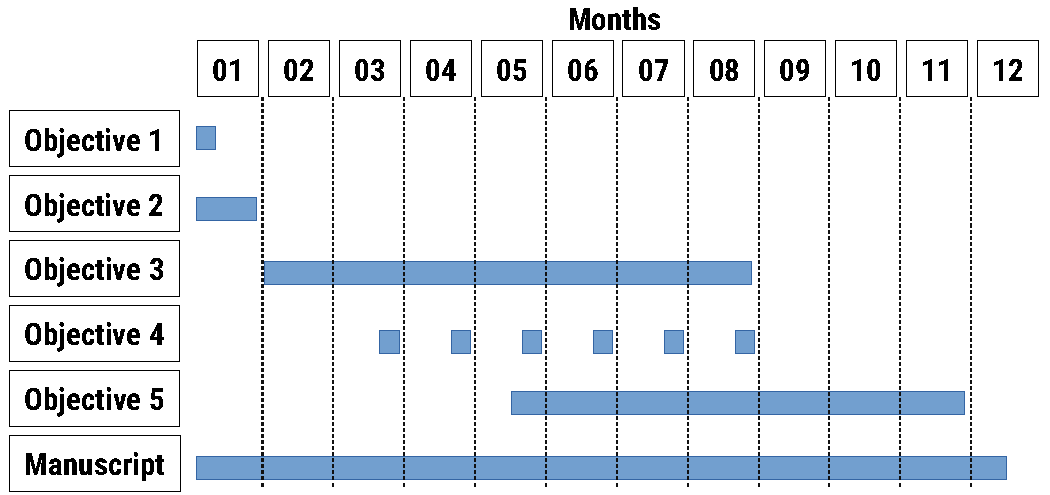
\includegraphics[scale=0.80]{figures/zzz-schedule.pdf}
\caption{Research Schedule}
\label{fig:schedule}
\end{center}
\end{figure}

%==================================================================================================%

\makereferences{cs-296-proposal}
\newpage

%==================================================================================================%

\begin{appendices}

%==================================================================================================%

\section{First Formal Framework (FF1)} \label{a-ff1}

%==================================================================================================%

\subsection{Multisets} \label{a-ff1-multiset}

\begin{enumerate}
   \item $V=\{a_1,...,a_k\}$ - alphabet.
   \item $M:V \rightarrow \mathbb{N}$ - multiset over $V$.
   \item $M(a)$ - number of occurrence of symbol $a$ in multiset $M$.
   \item $|M| = \sum_{a \in V} M(a)$ - size of multiset $M$.
   \item $a_1^{M(a_1)}...a_k^{M(a_k)}$ - string notation for multiset $M$.
   \item $supp(M) = \{a \in V | M(a) \geq 1\}$ - \emph{support} of multiset $M$.
   \item $\langle V, \mathbb{N}\rangle$ - set of \emph{finite} multiset over $V$.
   \item $M: V \rightarrow \mathbb{N} \cup \{\infty\}$ - a multiset over $V$ that allows infinite
         symbol occurrence.
   \item $\langle V, \mathbb{N}_{\infty} \rangle$ - set of \emph{possibly non-finite} multisets over
         $V$.
   \item $X \leq Y$ or $X \subseteq Y$ - multiset \emph{inclusion} relation or \emph{submultiset} 
         relation.
         \begin{itemize}
         \item $X$, $Y$ are multisets over $V$.
         \item $X(a) \leq Y(a)$, $\forall a \in V$
         \end{itemize}
   \item $Z = X + Y$ or $Z = X \cup Y$ - multiset \emph{union/addition}.
         \begin{itemize}
         \item $X, Y$ are multisets over $V$.
         \item $Z$ is the `sum' or `union' of multisets $X, Y$.
         \item $Z(a) = X(a) + Y(a)$, $\forall a \in V$
         \end{itemize}
   \item $Z = X - Y$ - multiset \emph{difference}.
         \begin{itemize}
         \item $X, Y$ are multiset over $V$.
         \item $X \geq Y$.
         \item $Z(a) = X(a) - Y(a)$, $\forall a \in V$ 
         \end{itemize}
   \item $X \leq Y$ - vector of multisets \emph{inclusion} relation.
         \begin{itemize}
         \item $X = (x_1,...,x_m)$. $X$ is a vector of multisets. $x_i$ is a multiset over $V$.
         \item $Y = (y_1,...,y_m)$. $Y$ is a vector of multisets. $y_i$ is a multiset over $V$.
         \item $x_i \leq y_i$, $\forall i, 1 \leq i \leq m$
         \end{itemize}
   \item $Z = X + Y$ or $Z = X \cup Y$ - vector of multisets \emph{addition}.
         \begin{itemize}
         \item $X = (x_1,...,x_m)$. $X$ is a vector of multisets. $x_i$ is a multiset over $V$.
         \item $Y = (y_1,...,y_m)$. $Y$ is a vector of multisets. $y_i$ is a multiset over $V$.
         \item $Z = (z_1,...,z_m)$. $Z$ is a vector of multisets. $z_i$ is a multiset over $V$.
         \item $z_i = x_i + y_i$, $\forall i, 1 \leq i \leq m$
         \end{itemize}
   \item $Z = X - Y$ - vector of multiset \emph{difference}.
         \begin{itemize}
         \item $X = (x_1,...,x_m)$. $X$ is a vector of multisets. $x_i$ is a multiset over $V$.
         \item $Y = (y_1,...,y_m)$. $Y$ is a vector of multisets. $y_i$ is a multiset over $V$.
         \item $Z = (z_1,...,z_m)$. $Z$ is a vector of multisets. $z_i$ is a multiset over $V$.
         \item $X \geq Y$.
         \item $z_i = x_i - y_i$, $\forall i, 1 \leq i \leq m$
         \end{itemize}

\end{enumerate}

%==================================================================================================%

\subsection{Network of Cells} \label{a-ff1-net-cells}

\begin{enumerate}
   \item $\Pi = (n, V, w, Inf, R)$ is the network of cells.
   \item $n$ is the number of cells.
   \item $V$ is the finite alphabet.
   \item $w = (w_1,...,w_n)$ is a vector of finite multisets over $V$.
         \begin{itemize}
         \item $w_i \in \langle V, \mathbb{N} \rangle$, $\forall i$, $1 \leq i \leq n$
         \item $w_i$ is the multiset associated with cell $i$.
         \end{itemize}
   \item $Inf = (Inf_1,...,Inf_n)$ - vector of subsets of $V$.
         \begin{itemize}
         \item $Inf_i \subseteq  V$.
         \item $Inf_i$ is the set of symbols occurring infinitely often in cell $i$.
         \end{itemize}
   \item $R$ is finite set of \emph{interactive rules}.
\end{enumerate}

%==================================================================================================%

\subsection{Interactive Rule} \label{a-ff1-rule}

\begin{enumerate}
   \item $(X \rightarrow Y; P, Q)$ is the form of an interactive rule.
   \item $X = (x_1,...,x_n)$ is a vector of multisets \emph{consumed} by the rule.
         \begin{itemize}
         \item $x_i$ is a multiset over $V$, $\forall i$, $1 \leq i \leq n$.
         \end{itemize}
   \item $Y = (y_1,...,y_n)$ is a vector of multisets \emph{produced} by the rule.
         \begin{itemize}
         \item $y_i$ is a multiset over $V$, $\forall i$, $1 \leq i \leq n$.
         \end{itemize}
   \item $P = (p_1,...,p_n)$ is a vector of sets of multisets. 
         \begin{itemize}
         \item $p_i$ is a set of multiset over $V$, $\forall i$, $1 \leq i \leq n$.
         \item $p_i$ contains all the required (`\emph{permitting}') multisets for cell $i$. 
         \end{itemize}
   \item $Q = (q_1,...,q_n)$ is a vector of sets of multisets.
         \begin{itemize}
         \item $q_i$ is a finite set of multiset over $V$, $\forall i$, $1 \leq i \leq n$.
         \item $q_i$ contains all the forbidden (`\emph{forbidding}') multisets for cell $i$. 
         \end{itemize}
   \item $X \rightarrow Y$ is the rewriting rule that rewrites of symbols in multisets $x_i$
         (in $X$) to symbols in multisets $y_j$ (in $Y$).
\end{enumerate}

%==================================================================================================%

\subsection{Configurations} \label{a-ff1-config} 

\begin{enumerate}
   \item $C = (u'_1,...,u'_n)$ is a vector of multisets known as a \emph{configuration} of $\Pi$.
         \begin{itemize}
         \item $u'_i \in \langle V, \mathbb{N}_{\infty} \rangle$, $\forall i$, $1 \leq i \leq n$.
         \end{itemize}
   \item $Inf^{\infty} = (Inf_1^{\infty},...,Inf_n^{\infty})$ (NOTE)
         \begin{itemize}
         \item Vector of infinite multisets.
         \item $Inf^{\infty}_i = b_1^{\infty}\cdots b_k^{\infty}$, $b_i \in Inf_i$, $\forall i$, $1 \leq i \leq k = |Inf_i|$ 
         \end{itemize}
   \item $C^{f} = (u_1,...,u_n)$
         \begin{itemize}
         \item Finite part of the configuration $C$.
         \item $u'_i = u_i + Inf_i^{\infty}$, $u_i \cap Inf_i = \emptyset$, $\forall i$, $1 \leq i \leq n$ 
         \item $u'_i = u_i + Inf_i^{\infty}$, $supp(u_i) \cap Inf_i = \emptyset$, $\forall i$, $1 \leq i \leq n$ (NOTE)
         \item $C^f_0 = w = (w_1,...,w_n)$ - finite parts of the initial configuration $C$.
         \item $C_0 = w + Inf^{\infty}$ - full initial configuration of $\Pi$.
         \end{itemize}

\end{enumerate}

%==================================================================================================%

\subsection{Eligibility of an Rule and Applicability of a Multiset of Rules} \label{a-ff1-eligible}

\begin{enumerate}
   \item $eligibe(r,C) \Leftrightarrow \forall i$, $(1 \leq i \leq n)$, $(x_i \subseteq u_i ),(\forall p \in p_i, p \subseteq u_i), (\forall q \in q_i, q \not\subseteq u_i)$
         \begin{itemize}
         \item Eligibility of rule $r$ with respect to configuration $C$.
         \item $C^f = (u_1,...,u_n)$ - vector of finite multisets ($u_i$). Multisets in the cells.
         \item $X = (x_1,...,x_n)$ - vector of multisets ($x_i$). Multisets to be `consumed'.
         \item $P = (p_1,...,p_n)$ - vector of multisets ($p_i$). Sets of required multisets for all cells.
         \item $Q = (q_1,...,q_n)$ - vector of multisets ($q_i$). Sets of required multisets for all cells.
         \end{itemize}
   \item $\exists j, x_j \cap (V - Inf_j) \neq \emptyset$
         \begin{itemize}
         \item There is at least one multiset $x_j$ in $X$  such that least one symbol appearing in $x_j$ has finite multiplicity.
         \end{itemize}
   \item $Eligible(\Pi, C) = \{r \in R | eligible(r,C)\}$
         \begin{itemize}
         \item Set of all eligible rules with respect to configuration $C$.
         \end{itemize}
\end{enumerate}

%==================================================================================================%

\subsection{Marking Algorithm} 

\begin{itemize}
   \item $r_i: (X_i \rightarrow Y_i; P_i, Q_i)$ - interaction rule.
   \item $X_i = (x_{i,1},...,x_{i,n})$ - vector of multisets.
   \item $X'_i = (x'_{i,1},...,x'_{i,n})$ - vector of multisets.
   \item $x_{i,j} = x'_{i,j} + Inf_{j}^{\infty}$. $x'_{i,j} \cap Inf_j = \emptyset$
   \item $C^f = (v_1,...,v_n)$ - vector of multisets. Finite part of the configuration.
   \item $R = \{r_1,...,r_h\}$ - set of eligible rules $r_i$.
   \item $R' \in \langle R, \mathbb{N} \rangle$ - finite multiset of eligible rules.
\end{itemize}

\begin{enumerate}
   \item $Mark_0(\Pi, C, R') = (\lambda,...,\lambda)$. $i = 1$.
   \item If $X'_i \leq (C^f - Mark_{i-1}(\Pi, C, R'))$
         \begin{itemize}
         \item \texttt{TRUE}: $Mark_i(\Pi, C, R') = (C^f - Mark_{i-1}(\Pi, C, R')) - X'_i$
         \item \texttt{FALSE}: return \texttt{false};
         \end{itemize}
   \item If $i=k$
         \begin{itemize}
         \item \texttt{TRUE}: return \texttt{true} and $Mark(\Pi, C, R') = Mark_k(\Pi, C, R')$
         \item \texttt{FALSE}: $i = i + 1$. Go back to step 2.
         \end{itemize}
\end{enumerate}

%==================================================================================================%

\subsection{Applicability of a Multiset of Rules} \label{a-ff1-applicable}

\begin{enumerate}
   \item $appl(R',C) \Leftrightarrow $ marking algorithm returns \texttt{true} and $Mark(\Pi, C, R')$.
         \begin{itemize}
         \item Applicability of multiset of rules $R'$ with respect to configuration $C$.
         \end{itemize}
   \item $Appl(\Pi, C) = \{R' \in \langle R, \mathbb{N} \rangle \s | \s R = Eligible(\Pi,C), appl(R',C) \}$
         \begin{itemize}
         \item Set of all applicable multisets of rules  with respect to configuration $C$.
         \end{itemize}
   \item $Apply(\Pi, C,R') = C - Mark(\Pi, C, R') + \sum_{i=1}^{k} Y'_i $
         \begin{itemize}
         \item A new configuration when rules in $R'$ are applied.
         \end{itemize}
\end{enumerate}

%==================================================================================================%

\subsection{Derivation Modes} \label{a-ff1-derive}

\begin{enumerate}
   \item $Appl(\Pi, C, \delta) \subseteq Appl(\Pi, C)$ 
         \begin{itemize}
         \item Set of applicable multisets of rules in $\delta$-mode.
         \end{itemize}
   \item $Appl(\Pi, C, asyn) = Appl(\Pi, C)$
         \begin{itemize}
         \item $\delta = asyn$. \textit{Asynchronous} mode.
         \end{itemize}
   \item $Appl(\Pi, C, sequ) = \{R' \in Appl(\Pi, C) \s | \s |R'|=1\}$
         \begin{itemize}
         \item $\delta = sequ$. \textit{Sequential} mode.
         \item Only one rule is applicable per step.
         \end{itemize}
   \item $Appl(\Pi, C, max) = \{R' \in Appl(\Pi, C) \s | \not\exists R'' \in Appl(\Pi, C), \s R' \not\subseteq R'' \}$
         \begin{itemize}
         \item $\delta = max$. \textit{Maximally parallel} mode.
         \item The multiset of rule $R'$ is maximal if by adding any (multiplicity of) rules will make the multiset of rules no longer applicable.
         \end{itemize}
   \item $Appl(\Pi, C, min) = \{R' \in Appl(\Pi, C) \s | \s \not\exists R'' \in Appl(\Pi,C), \s R' \subseteq R'', \exists j, (R''-R') \cap R_j \neq \emptyset, R' \cap R_j = \emptyset\}$
         \begin{itemize}
         \item $\delta = min$. \textit{Minimally parallel} mode.
         \item There should be at least one rule in $R'$ from each partition $R_j, \forall i, 1 \leq i \leq h$.
         \item $R = R_1 \cup R_2 \cup \cdots \cup R_h$. Rule set $R$ is be partitioned.
         \item $R' \subseteq R''$. $R''$ `extends' R'.
         \end{itemize}
   \item $\delta \in \{asyn, sequ, max, min\}$
         \begin{itemize}
         \item Basic derivation modes.
         \end{itemize}
   \item $Appl(\Pi, C, max_{rule}\delta) = \{R' \in Appl(\Pi, C, \delta) \s | \s \not\exists R'' \in Appl(\Pi,C, \delta) \s |R''| > |R'|\}$
         \begin{itemize}
         \item \textit{Maximum rules} $\delta$-mode.
         \item Multiset of rules in $\delta$-mode with maximum number of rule applications. 
         \end{itemize}
   \item $Appl(\Pi, C, max_{set}\delta) = \{R' \in Appl(\Pi, C, \delta) \s | \s \not\exists R'' \in Appl(\Pi,C, \delta) \s ||R''|| > ||R'||\}$
         \begin{itemize}
         \item \textit{Maximum set} $\delta$-mode.
         \item Multiset of rules in $\delta$-mode with maximum set of rules. 
         \end{itemize}
   \item $Appl(\Pi, C, all_{set}\delta) = \{R' \in Appl(\Pi, C, \delta) \s | \s \forall j, 1 \leq j \leq h, (R_j \cap \bigcup_{X \in Appl(\Pi,C)} X \neq \emptyset) \rightarrow (R_j \cap R' \neq \emptyset)\}$
         \begin{itemize}
         \item \textit{All set} $\delta$-mode.
         \item Multiset of rules in $\delta$-mode in which all partitions of the rule set contributes to $R'$. 
         \end{itemize}
\end{enumerate}

%==================================================================================================%

\subsection{Transitions} \label{a-ff1-transition}

\begin{enumerate}
   \item $C \Rightarrow_{(\Pi, \Delta)} C' \Leftrightarrow \exists R' \in Appl(\Pi,C,\Delta),\s C'=Apply(\Pi,C,R')$
         \begin{itemize}
         \item Transition in $\Delta$-mode.
         \end{itemize}
   \item $C \Rightarrow_{(\Pi, \Delta)}^{*} C'$
         \begin{itemize}
         \item Transitive closure and reflexive nature of the transition relation $\Rightarrow_{(\Pi,\Delta)}$
         \end{itemize}
   \item $accessible(C,\Pi, \Delta) \Leftrightarrow C_0 \Rightarrow_{(\Pi, \Delta)} C$
         \begin{itemize}
         \item Accessibility of configuration $C$ in $\Delta$-mode.
         \item $C_0$  is the initial configuration.
         \end{itemize}
   \item $Acc(\Pi, \Delta) = \{C \s | \s accessible(C, \Pi, \Delta)\}$ 
         \begin{itemize}
         \item Set of all accessible configurations using $\Delta$-mode derivation. 
         \end{itemize}
   \item $Deterministic(\Pi, \Delta) \Leftrightarrow \forall C \in Acc(\Pi, \Delta), Appl(\Pi, C, \Delta)| \leq 1$ 
         \begin{itemize}
         \item System $\Pi$ is deterministic with respect to $\Delta$-mode derivation.
         \end{itemize}
\end{enumerate}

%==================================================================================================%

\subsection{Halting Conditions} \label{a-ff1-halt}

\begin{enumerate}
   \item $H(\Pi, \Delta) = \{C' \in Acc(\Pi, \Delta) \s | \s Appl(\Pi, C', \Delta) = \emptyset\}$
         \begin{itemize}
         \item Set of \textit{total halting} configurations.
         \item Accessible configurations where there are no applicable multisets of rules.
         \end{itemize}
   \item $A(\Pi, \Delta) = \{C' \in Acc(\Pi, \Delta) \s | \s Appl(\Pi, C', \Delta) \neq \emptyset, \forall R' \in Appl(\Pi,C',\Delta), Apply(\Pi,C',R')=C' \}$
         \begin{itemize}
         \item Set of \textit{adult halting} configurations. 
         \item Accessible configurations where for all applicable rule $R'$ applying $R'$ to configuration $C'$ result to $C'$.
         \end{itemize}
   \item $h(\Pi, \Delta) = \{C' \in Acc(\Pi, \Delta) \s | \s \not\exists R' \in Appl(\Pi, C', \Delta), \forall i, 1 \leq i \leq h, R' \cap R_j \neq \emptyset \}$
         \begin{itemize}
         \item Set of \textit{partial halting} configurations. 
         \item Accessible configurations there are no multiset $R'$ of applicable rules such that $R'$ contains rules from all partions $R_j$.
         \end{itemize}
\end{enumerate}

% ================================================================================================ %

\section{Second Formal Framework (FF2)}\label{a-ff2}

% ================================================================================================ %

\subsection{Configurations} \label{a-ff2-config}

\begin{enumerate} 

\item $C = \{(i_1,w_1),...,(i_n,w_n)\}$ 

      \begin{itemize}
      \item A \textit{basic configuration} $C$ is a list of pairs $(i_j,w_j)$. Pairs $(i_j,w_j)$ are called \textit{cells}.
      \item $i_j \in \mathbb{N}$ is the \textit{id} of cell $j$. The id is unique per cell. i.e. $j \neq k \rightarrow i_j \neq i_k$. $[\forall j,k, 1 \leq j,k, \leq n]$
      \item $w_j \in O^*$ is the \textit{content} of some cell $j$.  $[\forall j, 1 \leq j \leq n]$
      \item $size(C)$ denotes the size of basic configuration $C$.
      \item $id(x)$ is a bijective function takes a cell ($x$) and returns the cell's id. 
      \item $id(j) = j$. For simplicity, the cell's position in the list is the same as its id.
      \end{itemize}

   \item $\mathbb{C} = \{ C \s | \s size(C) > 0\}$
         \begin{itemize}
         \item $\mathbb{C}$ is the set of all basic configurations with size greater than 0.
         \end{itemize}

\item $\mathcal{C} = (L, \rho) = (\{(i_1,l_1,w_1),...,(i_n,l_n,w_n)\}, \rho)$

      \begin{itemize}
      \item $\mathcal{C}$ is a configuration (where $C$  is a \textit{basic configuration}).
      \item $L =(i_1,l_1,w_1)...(i_n,l_n,w_n)$ is a list of \textit{labeled cells}.
      \item $l_j \in Lab$ is the \textit{label} of cell $j$ where $Lab$ is a set of \textit{labels}. $[\forall j, 1 \leq j \leq n]$
      \item Two cells can have the same label but not the same $id$.
      \item $\rho \subseteq \mathbb{N} \times \mathbb{N}$ is a relation the represents the connection between cells.
      \item $\mathcal{C}_m = L$ and $\mathcal{C}_\rho = \rho$.
      \item $\overline{\mathcal{C}}_m \in \mathbb{C}$ is the projection of $\mathcal{C}_m$ as basic (unlabeled) configuration.
      \end{itemize}

\item $\mathfrak{C} = \{\mathcal{C} \s | \s \mathcal{C} = (L, \rho)\}$
      \begin{itemize}
      \item $\mathfrak{C}$ is the set of all possible configurations.
      \end{itemize}

\end{enumerate}

% ================================================================================================ %

\subsection{Components of a Rule} \label{a-ff2-rule}

\begin{enumerate}
   \item $r = (Labels, \rho, Perm, For, Rewrite, Label\mn Rename, Delete, Delete\mn and\mn Move, Generate, Generate\mn and\mn Copy,\\ Change\mn Relation)$
         \begin{itemize}
         \item $r$ is a rule.
         \end{itemize}
   \item $Labels(r) = (l_1,...,l_k) \in Lab^k$ 
         \begin{itemize}
         \item $Label(r)$ is a list of cell labels that introduces $k$ \textit{virtual cells}.
         \item $k$ labels for virtual cells.
         \item $\mathbb{N}_k = \{1,...,k\}$.
         \item $\mathbb{C}_k \subseteq \mathbb{C}$ is the set of basic configurations, where the only allowed cell ids are in $\mathbb{N}_k$.
         \end{itemize}
   \item $\rho(r) \subseteq \mathbb{N}_k \times \mathbb{N}_k$
         \begin{itemize}
         \item $\rho(r)$ is a relation on virtual cells (e.g. indicating parent relation).
         \end{itemize}
   \item $Perm(r) \subseteq \mathbb{C}_k$
         \begin{itemize}
         \item $Perm(r)$ defines the permitting condition.
         \end{itemize}
   \item $For(r) \subseteq \mathbb{C}_k$
         \begin{itemize}
         \item $For(r)$ defines the forbidding condition.
         \end{itemize}
   \item $Rewrite(r) = U \rightarrow V$
         \begin{itemize}
         \item $U, V \in \mathbb{C}_k$
         \item $Rewrite(r)$ is a general rewriting rule, rewriting a finite basic configuration $U$ to another finite basic configuration $V$.
         \end{itemize}
   \item $Label\mn Rename(r) \in (\mathbb{N}_k \times Lab)^*$
         \begin{itemize}
         \item $Label\mn Rename(r)$ allows us to specify new labels for the cells whose index (or id) appears in the list.
         \end{itemize}
   \item $Delete(r) \in \mathbb{N}_k^*$
         \begin{itemize}
         \item $Delete(r)$ gives the indices of the virtual cells to be deleted.
         \end{itemize}
   \item $Delete\mn Move(r) \in (\mathbb{N}_k \times \mathbb{N}_k)^*$
         \begin{itemize}
         \item $Delete\mn Move(r)$ is a list of pairs of indices, e.g. $(i,j)$, that indicates that virtual cell $i$ should be deleted and its content should be moved to virtual cell $j$.
         \end{itemize}
   \item $Generate(r) \in (\mathbb{N}' \times Lab \times O^*)^*$
         \begin{itemize}
         \item $Generate(r)$ is a list of triples where each triple contains a \textit{primed} index, a label, and a multiset i.e. $(j', h, u)$.  
         \item This component introduces new cells (with \textit{primed} index) to be created when the rule is applied.
         \end{itemize}
   \item $Generate\mn Copy(r) \in (\mathbb{N}' \times Lab \times \mathbb{N} \times (O^* \times  O^*))^*$
         \begin{itemize}
         \item $Generate\mn Copy(r)$ is a list of quadruples where each quadruple contains a \textit{primed} index, a label, an index, and a rewriting rule i.e. $(j', h, i, u \rightarrow v)$.  
         \item Each tuple $(j', h, i, u \rightarrow v)$ means that a new cell should be created, having a new id $j'$ and the label $h$, by first copying every object inside cell $i$ and then applying the rewriting rule to contents of the new cell.
         \end{itemize}
   \item $Change\mn Relation$
         \begin{itemize}
         \item $Change\mn Relation$ is a \textit{graph transducer} that updates the relation $\rho$.
         \item This transducer should be recursive and it can only add and remove edges.
         \end{itemize}
\end{enumerate}

% ================================================================================================ %

\subsection{Eligibility of an Instance Vector} \label{a-ff2-eligible}
\begin{enumerate}
   \item $\bm{i} = (i_1,...,i_n) \in \mathbb{N}^n$ 
         \begin{itemize}
         \item An \textit{instance} $i$ is a vector of indices.
         \end{itemize}
   \item $C\langle \bm{i} \rangle = (\bm{i}|_{j_1}, w_1)...(\bm{i}|_{j_k}, w_k) = (i_{j_1},w_1)...(i_{j_k},w_k)$
         \begin{itemize}
         \item $C\langle \bm{i} \rangle$ is the \textit{instantiation} of basic configuration $C$ by instance $\bm{i}$.
         \item $C = (j_1,w_1)...(j_n,w_k) \in \mathbb{C}$.
         \item The set of cell ids$ \{j_1,...,j_k\}$ may not be equal to $\{1,...k\}$.
         \item $size(C) = k \leq |\bm{i}|$.
         \item Some cell ids ($j_q$) may be outside the range $[1,...,k = size(C)]$ but they are always in the range $[1,...,n]$.
         \item The id of cell $q$ is $j_q$. $\bm{i}|_{j_q}$ denotes the $j_q$-th index in vector/instance $\bm{i}$ which is $i_{j_q}$.
         \end{itemize}
   \item $r\langle \bm{i} \rangle$
         \begin{itemize}
         \item $r\langle \bm{i} \rangle$ is the instantiation of rule $r$ using instance $\bm{i}$.
         \item Replace all virtual ids $k$ by $\bm{i}|_k$ in all components of rule $r$ involving virtual ids (expect for parts $Labels(r)$ and $Generate(r)$).
         \end{itemize}
   \item $Eligible(\bm{i}, r, \mathcal{C})$ 
         \begin{itemize}
         \item $Eligible(\bm{i}, r, \mathcal{C})$ is the \textit{eligibility} of index vector $\bm{i}$ for instantiation for a rule $r$ in a configuration $\mathcal{C}$.
         \item $\bm{i} = (i_1,...,i_k) \in \mathbb{N}^k$.
         \item $r$ is a rule.
         \item $\mathcal{C} = (L,\rho)$.
         \item $Eligible(\bm{i},r,\mathcal{C})$ is true if the following conditions are true:
         \begin{itemize}
            \item Indices $i_j$ in index vector $\bm{i}$ are different from each other.
            \item $\forall j, 1 \leq j \leq k, 1 \leq i_j \leq size(\mathcal{C}), lab(i_j) = l_j$ where $Labels(r)= (l_1,...,l_k)$.
            \item $(j,m) \in \rho(r) \Rightarrow (i_j, i_m) \in \mathcal{C}_{\rho}$
         \end{itemize}
         \item $\mathcal{I}_{\mathcal{C}}(r) =\{\bm{i}\s |\s Eligible(\bm{i},r,\mathcal{C})\text{ is true}\}$.
         \end{itemize}
\end{enumerate}

% ================================================================================================ %

\subsection{Applicability of a Multiset of Rules}\label{a-ff2-applicable}
\begin{enumerate}
   \item $Applicable(R, \mathcal{C})$ 
         \begin{itemize}
         \item $Applicable(R,\mathcal{C})$ is the set of \textit{applicable} multisets of instantiated rules from $R$.
         \item $R = \{r_1,..,r_n\}$ is a multiset of rules. $r_i \neq r_j \in R$ are not necessarily different rules.
         \item $\mathcal{C} =(L, \rho)$ is a configuration. 
         \item $\mathcal{I}_{\mathcal{C}}(r_i) = \{v_{i,1},...,v_{i,k_i}\},\s \forall i, 1 \leq i \leq n$ where $v_{i,j_i}$ is an instance vector.
         \item $\{(r_1, v_{1,j_1}),...,(r_n,v_{n,j_n})\}$ is a multiset of instantiated rules.
         \item $\{(r_1, v_{1,j_1}),...,(r_n,v_{n,j_n})\}\in Applicable(R,\mathcal{C})$ if following 5 conditions are true:
         \end{itemize}
   \item $\forall i, 1 \leq i \leq n, \forall P, P \in (Perm(r_i) \cup DPerm(r_i)),\s P\langle v_{i,j_i} \rangle \subseteq \overline{\mathcal{C}}_m$
         \begin{itemize}
         \item $DPerm(r) = \{(i,u)\s |\s (j', h, i, u \rightarrow v) \in Generate\mn and\mn Copy(r)\}$
         \end{itemize}
   \item $\forall i, 1 \leq i \leq n, \forall Q, Q \in For(r_i), Q\langle v_{i,j_i} \rangle \not\subseteq \overline{\mathcal{C}}_m$
   \item $\bigcup_{i=1}^{n} Bound(r\langle v_{i,j_i}\rangle) \subseteq \overline{\mathcal{C}}_m$
         \begin{itemize}
         \item $Bound(r)$ is the left-hand side of the rewriting rule in the component $Rewrite(r)$.
         \item $Rewrite(r) = U \rightarrow V$
         \end{itemize}
   \item $\forall i,j,k,\s (s,l_1) \in Label\mn Rename(r_i\langle v_{i,j_i}\rangle)\s \& \s (s, l_2) \in Label\mn Rename(r_k \langle v_{k,j_k} \rangle) \rightarrow l_1 = l_2$ 
   \item Consecutive applications of $Change\mn Relation(r_i)$ and $Change\mn Relation(r_j)$ yields the same results regardless of order of applications for $1 \leq i,j \leq n$.
   \item $Applicable(\Pi, \mathcal{C}) = \bigcup_{Applicable(R, \mathcal{C})\neq \emptyset} Applicable(R,\mathcal{C})$
\end{enumerate}

% ================================================================================================ %

\subsection{Applying a Multiset of Rules} \label{a-ff2-apply}

\begin{enumerate}
   \item $L_1 = \{(i_1,l_1,w'_1)...(i_n,l_n,w'_n)\}$
         \begin{itemize}
         \item $$w'_j = w_j - \Bigg(\bigcup_{(r_k,v_k)\in RI} U_k |_j \Bigg) + \Bigg(\bigcup_{(r_k,v_k) \in RI } V_k|_j \Bigg)$$
         \item $RI = \{(r_1,v_1)...(r_n,v_n)\}$
         \item $\mathcal{C} = (\{(i_1,l_1,w_1)...(i_n,l_n,w_n)\},\rho)$ 
         \item $Rewrite(r_k\langle v_k \rangle) = U_k \rightarrow V_k$
         \item $U_k,V_k \in \mathbb{C}_k$
         \end{itemize}

   \item $L_2 = \{(i_1,l'_1,w'_1)...(i_n,l'_n,w'_n)\}$
         \begin{itemize}
         \item \[ l'_j = \begin{cases} 
                         e_s, & \text{if } \exists(r_k,v_k)\in RI \text{ such that } (j,e_s) \in Label\mn Rename(r_k\langle v_k\rangle)\\
                         l_j, & \text{otherwise} 
                         \end{cases}\] 
        \end{itemize}

   \item $L_c = L_c(r_1) \cdot \cdots \cdot L_c(r_n)$
         \begin{itemize}
         \item $L_c(r_k) = \{(m_1, h_1, u_1)\cdots (m_t,h_t,u_t)\}$
         \item $Generate(r_k) = \{(1', h_1, u_1) \cdots (t', h_t, u_t)\}$
         \end{itemize}

   \item $L'_c = L'_c(r_1)\cdot \cdots \cdot L'_c(r_n)$
         \begin{itemize}
         \item $L'_c(r_k) = \{(m_{t+1},e_1, w'_{n_1} - u_1 + v_1)...(m_{t+s}, e_s, w'_{n_s} - u_s + v_s)\}$
         \item $Generate\mn and \mn Copy(r_k) = \{(1',e_1, n_1, u_1 \rightarrow v_1)...(s', e_s, n_s, u_s \rightarrow v_s)\}$
         \item $(i_j, l'_j, w'_j) \in L_2$
         \end{itemize}

   \item $L_3 = L_2 \cdot  L_c \cdot L_c'$
   \item $L_4 = \{(i_1, l_1', w_1'') \cdots (i_n, l_n', w_n'')\}$
         \begin{itemize}
         \item $$w_j'' = w_j' + \Bigg(\bigcup_{\text{last}(i_k)=i_j} w_k' \Bigg)$$
         \item $(i_j, l_j', w_j') \in L_3$
         \item $\textbf{p} = (p_1,...,p_j,...,p_n)$ - vector of ``destination" cell ids for multisets from cells that may be deleted.
         \item $p_j = p(i_j)$ - destination cell for multiset from cell $i_j$. 
         \item \[ p(i_j) = \begin{cases} 
                           *  , & \text{if } \exists(r_k,v_k)\in RI \text{ such that } i_j \in Delete(r_k\langle v_k\rangle)\\
                           e  , & \text{if } \exists(r_k,v_k)\in RI \text{ such that } (i_j,e) \in Delete\mn and\mn Move(r_k\langle v_k\rangle)\\
                           i_j, & \text{otherwise} 
                           \end{cases}\] 
         \item $Delete(r) \in \mathbb{N}_k^*$ is the list of cell ids to be deleted.
         \item $Delete\mn and\mn Move(r) \in (\mathbb{N}_k \times \mathbb{N}_k)^*$. $(i,j) \in Delete\mn and\mn Move(r)$ means to delete cell $i$ and move its multiset to
               cell $j$.
         \item If $p_k = p(i_k) = i_k$, then cell $i_k$ will not be deleted.
         \item If $p_k = p(i_k) \neq i_k$ (either $p(i_k)= *$ or $p(i_k)=e$), then cell $i_k$ will be deleted.
         \item If $p_k = i_k$, then there is a sequence $x_1,...,x_{j-1},...,x_m$ of cell ids where:
               \begin{itemize}
                  \item $x_1 = p_k$
                  \item $x_j = p(x_{j-1})$ for $2 \leq j \leq m$
                  \item $x_m = z$ 
               \end{itemize}
               There is a chain of ``delete-and-move" and $z$ is the last cell id to not be deleted or to be deleted and not moved.
         \item $last(i_j) = z$
         \end{itemize}
   \item $L_5 = \{(i_1,l_1',w_1'')...(i_{n_1},l_{n_1}',w_{n_1}'')\}$ where $(i_j,l_j',w_j'') \in L_4$ and $p_j = i_j$. 
         \begin{itemize}
         \item $L_5$ contains $L_4$ cells with the deleted cells removed.
         \end{itemize}
   \item $Apply(RI,\mathcal{C}) = (L_2, \mathcal{C}_{\rho}')$
         \begin{itemize}
         \item $\mathcal{C}_{\rho}'$ is the updated `parent' relation after $CREATE\mn NODES$, $DELETE\mn NODES$, and\\ $Change\mn Relation(r_k\langle v_k\rangle)$ have been computed
               for all $(r_k,v_k) \in RI$ on $\mathcal{C}_{\rho}$.
         \end{itemize}
\end{enumerate}

%==================================================================================================%

\section{Additional Notions in the Third Formal Framework (FF3)} \label{a-ff3}

%==================================================================================================%

\begin{enumerate}
   \item $X \ra Y; E$ is a form of the interaction rule. \label{a-ff3-rule}
         \begin{itemize}
         \item $X = (x_1,...,x_n)$ is a vector of multisets that the rule will consume. $x_i$ is the
               multiset that will be consumed from cell $i$.
         \item $Y = (y_1,...,y_n)$ is a vector of multisets that the rule will produce. $y_i$ is the
               multiset that will be produced at cell $i$.
         \item $E = (E_1,...,E_n)$ is a vector of regular expressions over the alphabet $V$ of the 
               system. $E_i$ is a regular expression over $V$. It defines the \emph{permitting 
               condition} related to cell $i$. $L(E_i)$ is the language defined by regular
               expression $E_i$ while $L^{\circ}(E_i)$ is the regular multiset language define by
               the regular expression $E_i$.
         \end{itemize}
   \item $\Pi = (n, V, w, c_in, c_ou, Inf, R)$ is the network of cells. It has the same components
         as the network of cells in FF1 (see Appendix \ref{a-ff1-config}) except for the additional
         $c_{in}$ and $c_{out}$ components specifying the input cells and the output cells 
         respectively. \label{a-ff3-net-cells}
   \item $Input: \mathbb{N} \times 2^{V} \ra V^n$ (probably should be $Input: \mathbb{N} \times 
         2^{\mathbb{N}}\ra \langle V, \mathbb{N}\rangle^n$) is an \emph{input function}. 
         \label{a-ff3-input}
         \begin{itemize}
         \item $Input(t,c) \in \langle V, \mathbb{N}\rangle^n$ is a size $n$ vector of multisets 
               that represents the input to the system which can be added to the configuration of 
               the system. $t \in \mathbb{N}$ is the time (step) while $c \in 2^{\mathbb{N}}$ is the
               set of `ids' of the input cells.
        \end{itemize}
   \item $\pi(S,X): 2^{\mathbb{N}} \times (\langle V, \mathbb{N}\rangle)^n \ra  (\langle V, 
         \mathbb{N}\rangle)^n$ (original: $2^{\mathbb{N}} \times \langle V,\mathbb{N}\rangle \ra
         \langle V,\mathbb{N}\rangle$) is a \emph{keeping function}. \label{a-ff3-keep}
         \begin{itemize} 
            \item $\pi$ takes a set of cell ids $S\in 2^{\mathbb{N}}$ and a vector of multiset 
                  $X = (X_1,...,X_i,...,X_n)$ and zero-out all the multisets $X_i$ if $i \not\in S$.
            \item $\pi(S,X) = (X'_1,...,X'_i,...,X'_n)$ where $X'_i = X_i$ if $i \in S$ otherwise 
                  $X'_i = 0$ if $i \not\in S$.
         \end{itemize}
   \item $Output: \mathbb{N} \times NC \times (V^n)^* \times 2^V \times \Delta \ra S$ is an 
         \emph{output function}. \label{a-ff3-out}
         \begin{itemize}
            \item The output function $Output$ takes the following as parameters: (1) the time $t 
                  \in \mathbb{N}$, (2) a system $\Pi \in NC$ where $NC$ is the set of \emph{network
                  of cells}, (3) a configuration history $C(t) \in (\langle V,N \rangle^n)^*$ 
                  (originally $(V^n)^*$) where $C(t) = C_0,...,C_t$, (4) a set of ids of the output
                  cells $c_{out} \in 2^{\mathbb{N}}$ (originally $2^V$), a derivation mode $\delta 
                  \in \Delta$.
            \item The output function then returns $Output(t, \Pi, C(t), c_{out}, \delta)$ which is
                  a size $n$ vector of multisets that represent the output of the system at time 
                  $t$. The $Output$ function uses the keeping function $\pi$.
            \item $Output(t, \Pi, C(t), c_{out}, \delta) = \pi(c_{out},C_t)$ if $Applicable(\Pi,
                  C_t, \delta) = \emptyset$ (if there are not more applicable multisets of rules).
                  Otherwise, $Output(t, \Pi, C(t), c_{out}, \delta) = \emptyset$.
         \end{itemize}
\end{enumerate}


\end{appendices}

%==================================================================================================%

\end{document}





















